\section{Tugas 2 -- Deteksi Fraud}
Data latih berisi 403.077 transaksi Januari--Agustus 2025 dengan tingkat fraud \TduaFraudRate\%; data uji 106.674 transaksi September--Oktober.
Skor dipakai \emph{sebelum} transaksi diproses, dan setiap transaksi yang ditandai berbiaya Rp~25.000.

\subsection*{(a) Audit label dan fitur}
\textbf{Label belum matang.} Label \texttt{is\_fraud} berarti ``terkonfirmasi fraud saat data ditarik (31 Agustus)''. Tingkat fraud mingguan stabil
di sekitar \TduaRateDasarMingguan\% lalu turun tajam di akhir data hingga \TduaRateMingguTerakhir\% pada minggu terakhir (Gambar~\ref{fig:t2label}):
fraud yang baru terjadi belum sempat dilaporkan sehingga masih berlabel 0. Batas label matang diestimasi otomatis sebagai minggu pertama
yang tingkat fraudnya < 80\% median Januari--Juli: \textbf{\TduaBatasMatang}.

\textbf{Fitur yang tidak tersedia saat transaksi.} \texttt{flag\_review\_manual} memiliki AUC tunggal \TduaReviewAUC: tingkat fraud
\TduaReviewFraudJikaSatu\% pada transaksi yang pernah direview, dan \TduaReviewPorsiFraud\% seluruh fraud pernah direview.
Review dilakukan \emph{setelah} transaksi dicurigai, dan tingkat review di data uji (\TduaReviewRateTest\%) lebih rendah daripada di data latih
(\TduaReviewRateTrain\%) karena sebagian review belum terjadi. Memasukkan fitur ini menaikkan PR-AUC validasi dari \TduaPRAUCBersih{} menjadi
\TduaPRAUCReview{} --- kenaikan semu yang tidak akan terulang di produksi (Tabel~\ref{tab:t2_audit_dampak}). \texttt{v15} naik lurus setiap bulan
(penanda waktu). Keduanya dibuang. Nilai kosong \texttt{menit\_sejak\_trx\_terakhir} dan \texttt{rasio\_nominal\_rata2} (±25\%) terbukti selalu
bersamaan dan menandai transaksi pertama pengguna, sehingga dipertahankan sebagai informasi.

\begin{figure}[ht]\centering
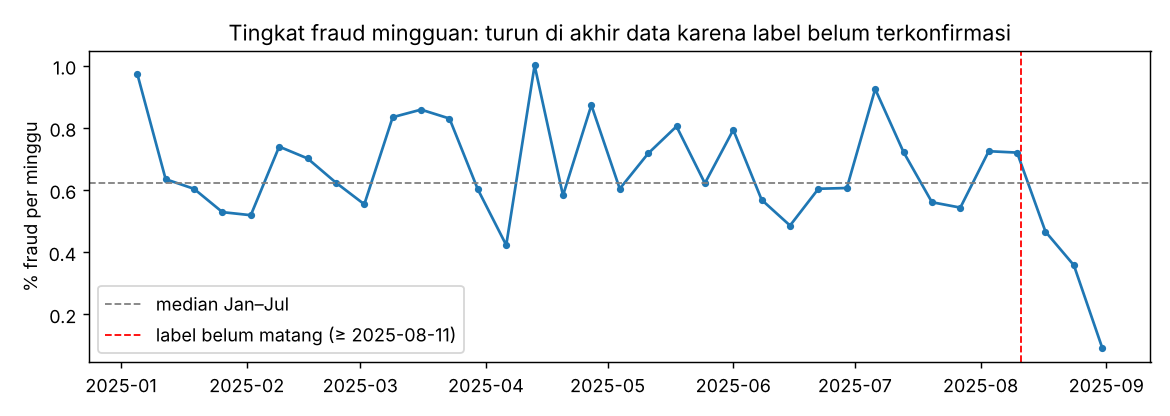
\includegraphics[width=.85\linewidth]{t2_audit_label.png}
\caption{Tingkat fraud mingguan; garis merah = awal periode label belum matang.}\label{fig:t2label}
\end{figure}
\begin{table}[ht]
\centering\small
\begin{tabular}{lrr}
\toprule
varian & pr\_auc & roc\_auc \\
\midrule
tanpa fitur bermasalah (dipakai) & 0.781 & 0.991 \\
+ flag\_review\_manual & 0.917 & 0.997 \\
+ v15 & 0.781 & 0.991 \\
\bottomrule
\end{tabular}
\caption{Dampak fitur bermasalah (fold F2: latih Jan–Mei, val Jun–Jul).}
\label{tab:t2_audit_dampak}
\end{table}


\subsection*{(b) Validasi berbasis waktu dan label yang belum lengkap}
Setiap fold terdiri dari periode latih, satu bulan kalibrasi, dan dua bulan validasi: F1 (latih Jan--Mar, kalibrasi Apr, validasi Mei--Jun) dan
F2 (latih Jan--Apr, kalibrasi Mei, validasi Jun--Jul). Periode validasi sengaja dipilih yang labelnya sudah matang; minggu-minggu akhir Agustus
tidak pernah dipakai sebagai validasi karena fraud-nya belum lengkap dan akan membuat metrik bias.
Random stratified CV memberi PR-AUC \TduaValRandomPR{} dibanding \TduaValWaktuPR{} pada skema waktu (Tabel~\ref{tab:t2_validasi}).

Untuk data latih, kami mensimulasikan kondisi 31 Agustus pada fold F2: fraud di tiga minggu terakhir data latih disembunyikan dengan proporsi
yang sama seperti yang teramati di Agustus, lalu dibandingkan (i) memakai label apa adanya dan (ii) membuang periode belum matang
(Tabel~\ref{tab:t2_label_lag}). Keputusan untuk model final: \textbf{\TduaKonfigLabel} periode belum matang (data latih final sampai \TduaBatasLatih).
Fitur historis berbasis label juga hanya memakai label yang berumur > 30 hari.

\begin{table}[ht]
\centering\small
\resizebox{\ifdim\width>\linewidth\linewidth\else\width\fi}{!}{%
\begin{tabular}{lrrrr}
\toprule
strategi & pr\_auc & roc\_auc & rata2\_prob\_val & fraud\_tersembunyi \\
\midrule
label lengkap (acuan, tidak realistis) & 0.781 & 0.991 & 0.005 & 138 \\
label belum matang dipakai apa adanya & 0.775 & 0.991 & 0.004 & 138 \\
buang periode belum matang (dipakai) & 0.776 & 0.991 & 0.005 & 138 \\
\bottomrule
\end{tabular}
}
\caption{Simulasi label belum matang pada 3 minggu terakhir data latih (fold F2).}
\label{tab:t2_label_lag}
\end{table}


\subsection*{(c) Fitur perilaku tanpa informasi masa depan}
Data latih dan uji digabung lalu diurutkan menurut waktu; setiap fitur hanya memakai transaksi \emph{sebelum} transaksi tersebut.
Fitur pengguna: rata-rata dan z-score log-nominal terhadap riwayatnya, rasio terhadap nominal maksimum sebelumnya, merchant/kategori baru,
jumlah transaksi 1 jam dan 24 jam (hitungan sendiri), jeda sejak transaksi sebelumnya, porsi transaksi malam. Fitur merchant: rasio nominal
terhadap rata-rata merchant, volume 24 jam dan 7 hari, pengguna baru. Tingkat fraud historis merchant dan pengguna dihitung hanya dari label yang
sudah matang (> 30 hari sebelumnya), dengan smoothing. Tiga tes otomatis memastikan tidak ada kebocoran: fitur masa lalu tidak berubah jika data
atau label masa depan diubah, dan hitung ulang manual cocok. Fitur perilaku menaikkan PR-AUC rata-rata dari \TduaPRTanpaPerilaku{} menjadi
\TduaPRPerilaku{} (Tabel~\ref{tab:t2_fitur_perilaku}).

\begin{table}[ht]
\centering\small
\begin{tabular}{lrr}
\toprule
fitur & pr\_auc & roc\_auc \\
\midrule
+ fitur perilaku (dipakai) & 0.787 & 0.990 \\
tanpa fitur perilaku buatan & 0.763 & 0.985 \\
\bottomrule
\end{tabular}
\caption{Dampak fitur perilaku buatan (rata-rata F1–F2).}
\label{tab:t2_fitur_perilaku}
\end{table}


\subsection*{(d) Ketidakseimbangan kelas}
Dibandingkan baseline regresi logistik (PR-AUC \TduaPRLogreg) dan LightGBM dengan empat strategi: tanpa penanganan, \textit{class weight}
(\texttt{scale\_pos\_weight} = $\sqrt{\text{neg}/\text{pos}}$), \textit{undersampling} negatif 1:20, dan SMOTE 1:10 (hanya pada data latih fold).
Karena reweighting dan resampling menggeser probabilitas, setiap varian dikalibrasi isotonic di bulan kalibrasi sebelum aturan biaya diterapkan.
Pendekatan keempat, \textit{threshold tuning}, dibandingkan sebagai kolom ``biaya threshold tunggal'' (Tabel~\ref{tab:t2_imbalance}).
Terpilih: \textbf{\TduaKonfigImbalance} (biaya validasi terendah).

\begin{table}[ht]
\centering\small
\resizebox{\ifdim\width>\linewidth\linewidth\else\width\fi}{!}{%
\begin{tabular}{lrrrrrrr}
\toprule
strategi & pr\_auc & roc\_auc & biaya aturan (juta Rp) & biaya thr tunggal (juta Rp) & recall & presisi & ece\_mentah \\
\midrule
tanpa penanganan & 0.775 & 0.988 & 69.484 & 81.291 & 0.693 & 0.371 & 0.002 \\
undersampling negatif 1:20 & 0.760 & 0.988 & 71.514 & 83.972 & 0.685 & 0.354 & 0.002 \\
class weight (scale\_pos\_weight) & 0.769 & 0.989 & 72.333 & 82.470 & 0.684 & 0.386 & 0.001 \\
SMOTE (rasio 1:10) & 0.769 & 0.986 & 73.953 & 87.238 & 0.685 & 0.363 & 0.001 \\
Logistic regression (baseline) & 0.566 & 0.931 & 128.265 & 157.154 & 0.533 & 0.356 & 0.001 \\
\bottomrule
\end{tabular}
}
\caption{Strategi class imbalance (rata-rata F1–F2). Probabilitas dikalibrasi isotonic di bulan kalibrasi sebelum aturan biaya.}
\label{tab:t2_imbalance}
\end{table}


\subsection*{(e) Pergeseran pola}
Tingkat fraud per kanal berubah dari bulan ke bulan (Gambar~\ref{fig:t2drift}). \textit{Adversarial validation} (Juni--Agustus vs data uji)
menunjukkan model dapat membedakan keduanya dengan AUC \TduaAdvAUCSebelum{}; penyebab utamanya fitur kumulatif sejak Januari (jumlah transaksi,
tingkat fraud kategori kumulatif) yang nilainya naik terus mengikuti waktu. Setelah fitur tersebut dibuang, AUC adversarial turun menjadi
\TduaAdvAUC{} dengan PR-AUC hampir tidak berubah (Tabel~\ref{tab:t2_adversarial}). Adaptasi terhadap pergeseran dibandingkan pada fold F2:
seluruh data, tiga bulan terakhir saja, dan bobot waktu dengan paruh 60 hari (Tabel~\ref{tab:t2_adaptasi}); terpilih \textbf{\TduaKonfigAdaptasi}.

\begin{figure}[ht]\centering
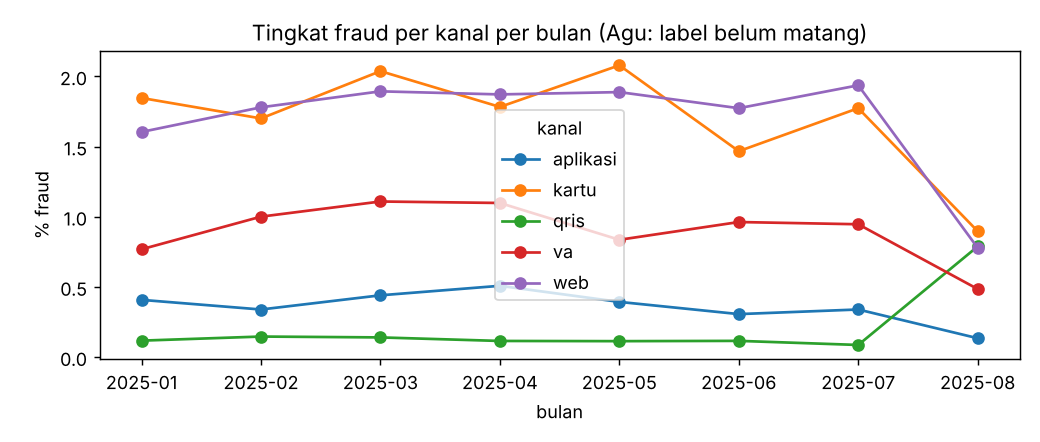
\includegraphics[width=.75\linewidth]{t2_drift_kanal.png}
\caption{Tingkat fraud per kanal per bulan.}\label{fig:t2drift}
\end{figure}
\begin{table}[ht]
\centering\small
\begin{tabular}{lrr}
\toprule
fitur & AUC adversarial (train vs test) & PR-AUC F2 \\
\midrule
dengan fitur kumulatif & 0.985 & 0.784 \\
tanpa fitur kumulatif (dipakai) & 0.873 & 0.781 \\
\bottomrule
\end{tabular}
\caption{Adversarial validation (Jun–Agu vs test Sep–Okt) sebelum/sesudah membuang fitur kumulatif.}
\label{tab:t2_adversarial}
\end{table}

\begin{table}[ht]
\centering\small
\begin{tabular}{lrr}
\toprule
adaptasi & pr\_auc & roc\_auc \\
\midrule
semua data latih & 0.781 & 0.991 \\
3 bulan terakhir saja & 0.769 & 0.990 \\
bobot waktu (paruh 60 hari) & 0.777 & 0.991 \\
\bottomrule
\end{tabular}
\caption{Adaptasi terhadap pergeseran pola (fold F2).}
\label{tab:t2_adaptasi}
\end{table}


\subsection*{(f) Kalibrasi dan aturan keputusan berbasis biaya}
Jika transaksi ditandai, biayanya Rp~25.000 (fraud tertahan tanpa kerugian); jika tidak, ekspektasi kerugiannya $p \times \text{nominal}$.
Maka transaksi ditandai bila $p \times \text{nominal} > 25.000$. Aturan ini hanya benar bila $p$ terkalibrasi, sehingga dibandingkan tanpa kalibrasi,
Platt (sigmoid), dan isotonic pada bulan kalibrasi (Tabel~\ref{tab:t2_kalibrasi_biaya}, Gambar~\ref{fig:t2rel}); terpilih \textbf{\TduaKonfigKalibrasi}.
Rata-rata biaya validasi per dua bulan: aturan kami Rp~\TduaBiayaAturan{} juta (recall \TduaRecallAturan\%), threshold tunggal Rp~\TduaBiayaThr{} juta,
menandai semua Rp~\TduaBiayaSemua{} juta, dan tidak menandai sama sekali Rp~\TduaBiayaTidak{} juta.

\begin{table}[ht]
\centering\small
\resizebox{\ifdim\width>\linewidth\linewidth\else\width\fi}{!}{%
\begin{tabular}{lrrrrrr}
\toprule
kalibrasi & brier & ece & biaya\_aturan\_p\_x\_nominal & biaya\_threshold\_tunggal & biaya\_tandai\_semua & biaya\_tidak\_menandai \\
\midrule
isotonic & 0.0023 & 0.0003 & 69.4844 & 81.2908 & 2567.6875 & 832.4982 \\
none & 0.0024 & 0.0018 & 83.1257 & 81.3297 & 2567.6875 & 832.4982 \\
sigmoid & 0.0022 & 0.0002 & 69.1319 & 81.3297 & 2567.6875 & 832.4982 \\
\bottomrule
\end{tabular}
}
\caption{Kalibrasi (Brier, ECE) dan biaya (juta Rp) di validasi, rata-rata F1–F2.}
\label{tab:t2_kalibrasi_biaya}
\end{table}

\begin{figure}[ht]\centering
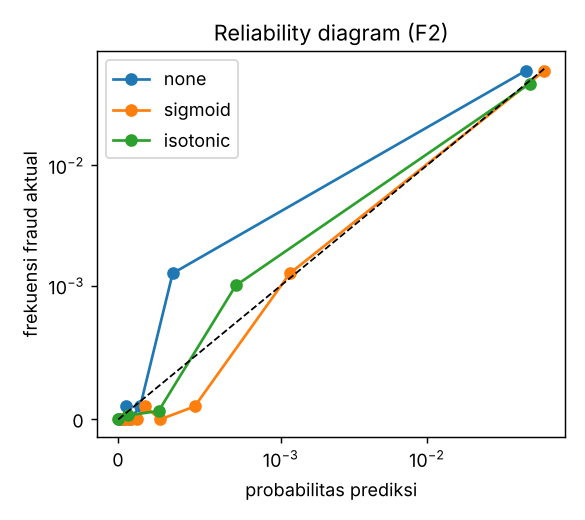
\includegraphics[width=.45\linewidth]{t2_reliability.png}
\caption{Reliability diagram fold F2 (skala log).}\label{fig:t2rel}
\end{figure}

\subsection*{(g) Analisis error}
Pada fold F2 model final mencapai PR-AUC \TduaFinalValPR{} dengan biaya Rp~\TduaFinalValBiaya{} juta, yang sebagian besar berasal dari fraud lolos
senilai Rp~\TduaNominalFN{} juta. Kanal dengan biaya terbesar adalah \textbf{\TduaKanalBiayaTerbesar} (recall \TduaKanalRecall\%)
(Tabel~\ref{tab:t2_breakdown_kanal}). Pola fraud yang ditemukan beserta recall model per pola ada di Tabel~\ref{tab:t2_pola_fraud};
pola dengan porsi terbesar adalah \emph{akun baru ($<$30 hari)}, yaitu 13{,}8\% dari seluruh fraud, tetapi recall model pada pola ini hanya 0{,}48. Dugaan kami, akun baru belum punya riwayat transaksi, sehingga fitur perilaku berbasis riwayat (rata-rata dan frekuensi sebelumnya) belum informatif. Recall terendah ada pada \emph{card testing} (0{,}37): nominalnya kecil ($<$Rp50 ribu), sehingga dengan aturan biaya kerugian per transaksi yang lolos rendah dan banyak yang berada di bawah threshold. Sebaliknya, pola pengambilalihan akun dan kartu tidak hadir jarak jauh tertangkap dengan baik (recall $\geq$0{,}95) karena sinyalnya kuat dan jelas.
\begin{table}[ht]
\centering\small
\resizebox{\ifdim\width>\linewidth\linewidth\else\width\fi}{!}{%
\begin{tabular}{lrrrrrrrrr}
\toprule
kanal & n & n\_fraud & rate\_fraud\_\% & pr\_auc & recall & FN & FP & nominal\_FN\_juta & biaya\_juta \\
\midrule
aplikasi & 45765 & 148 & 0.32 & 0.65 & 0.58 & 62 & 327 & 10.32 & 20.64 \\
kartu & 12676 & 206 & 1.63 & 0.83 & 0.71 & 60 & 154 & 9.08 & 16.58 \\
qris & 22714 & 23 & 0.10 & 0.08 & 0.22 & 18 & 130 & 9.20 & 12.57 \\
va & 15194 & 145 & 0.95 & 0.81 & 0.88 & 18 & 136 & 4.31 & 10.88 \\
web & 6360 & 118 & 1.86 & 0.91 & 0.75 & 30 & 60 & 2.63 & 6.33 \\
\bottomrule
\end{tabular}
}
\caption{Error per kanal (fold F2, aturan biaya).}
\label{tab:t2_breakdown_kanal}
\end{table}

\begin{table}[ht]
\centering\small
\resizebox{\ifdim\width>\linewidth\linewidth\else\width\fi}{!}{%
\begin{tabular}{lrrrr}
\toprule
pola & n\_trx & rate\_fraud\_\% & porsi\_dari\_semua\_fraud\_\% & recall\_model \\
\midrule
akun baru (< 30 hari) & 3551 & 2.48 & 13.75 & 0.48 \\
akses dari IP luar negeri & 861 & 9.06 & 12.19 & 0.68 \\
pengambilalihan akun (ganti password 7h + perangkat baru) & 131 & 51.15 & 10.47 & 0.96 \\
card testing ($\geq$3 trx/1 jam, nominal < 50rb) & 511 & 11.15 & 8.91 & 0.37 \\
kartu tidak hadir + jarak jauh (> 500 km) & 296 & 7.09 & 3.28 & 0.95 \\
merchant refund tinggi (> 10\%) & 31 & 12.90 & 0.62 & 1.00 \\
\bottomrule
\end{tabular}
}
\caption{Pola fraud: tingkat fraud dalam pola, porsi dari seluruh fraud, dan recall model (F2).}
\label{tab:t2_pola_fraud}
\end{table}


\textbf{Prediksi uji.} Model final dilatih sampai \TduaBatasLatih; pada data uji \TduaTestDitandai{} transaksi (\TduaTestPersenDitandai\%) ditandai
untuk direview, dengan rata-rata probabilitas \TduaTestProbRata\%.
